\chapter{Cubic Splines and their derivatives}
\label{chap:csplines}
Throughout the present analysis we occasionally use cubic splines for smoothing distributions, by fitting $y_i$ for a fixed set of $(x_i, y_i)$ tuples and calculating a spline between these points.
Typically, each $y_i$ can be associated with an uncertainty and in order to propagate this uncertainty to the resulting spline fit, the derivatives of a spline function are needed.
Due to the lack of available implementations for this specific problem, we roll out our own implementation of cubic splines, based on the theory described below.

Splines are a model independent way to interpolate between grid points.
Cubic splines realize this interpolation with polynomial pieces of the form
\begin{equation*}
    f_i(t) = a_i + b_i t + c_i t^2 + d_i t^3 \quad \text{for } i=1 \ldots k \,,
\end{equation*}
where $t$ is a parameter $t \in [0,1]$.
For $n= k+1$ grid points $(x_0, y_0),\ldots,(x_k, y_k)$ there are $k$ polynomial pieces $f_i$.
Each parameter $t$ maps for the polynomial piece $f_i$ from the interval $t \in [0,1]$ to $x \in [x_i,x_{i+1}]$
\begin{equation*}
    t = t(x) = \frac{x-x_i}{x_{i+1}-x_i}
\end{equation*}
such that 
\begin{equation*}
    f(x) =
    \begin{cases}
        f_1(t) & \text{for }x \in [x_0,x_1] \\
        \vdots \\
        f_k(t) & \text{for }x \in [x_{k-1},x_k]
    \end{cases}
\end{equation*}
has a gapless coverage on $[x_0,x_k]$.
Each polynomial piece brings $4$ \gls{dof}.
Following Ref.~\cite{splines} these \gls{dof} are fixed by simultaneously satisfying the following set of constraints:
\begin{itemize}[itemsep=2pt,parsep=2pt]
    \item $f_i(0) = y_i$ for $i=1 \ldots k\,$,
    \item $f_i(1) = y_{i+1}$ for $i=1 \ldots k\,$,
    \item $f'_i(1) = f'_{i+1}(0)$ for $i=1 \ldots (k-1)\,$,
    \item $f''_i(1) = f''_{i+1}(0)$ for $i=1 \ldots (k-1)$ and,
    \item $f''_1(0) = f''_k(1) = 0$ (natural splines).
\end{itemize}
These are $k + k + (k-1) + (k-1) + 2 = 4k$ relations that constrain all $4k$ coefficients $a_i$, $b_i$, $c_i$ and $d_i$.
The latter relation defines \textit{natural} (cubic) splines and is a boundary condition.
Other common boundary conditions are:
\begin{itemize}[itemsep=2pt,parsep=2pt]
    \item \textit{not-a-knot}: The third derivative is also continuous at $(x_1, y_1)$ and $(x_k, y_k)$.
    \item \textit{periodic}: The interpolated functions is assumed to be periodic, i.e. $(x_0, y_0) \equiv (x_n, y_n)$.
    \item \textit{clamped}: The first derivative at curve ends are zero.
\end{itemize}
The coefficients $a_i, b_i, c_i$ and $d_i$ are unambiguously defined by the given set of grid points $y_0,\ldots,y_k$:
\begin{align*}
    a_i &= y_i \,, \\
    b_i &= D_i \,, \\
    c_i &= 3(y_{i+1} - y_{i}) - 2D_i - D_{i+1} \,, \\
    d_i &= 2(y_i - y_{i+1}) + D_i + D_{i+1} \,,
\end{align*}
with $D_i := f'_i(0)$.
This set of equations translates into solving the matrix equation
\begin{equation*}
    \underbrace{\begin{pmatrix}
        2 & 1 \\
        1 & 4 & 1 \\
        & 1 & 4 & 1 \\
        & & 1 & 4 & 1 \\
        & & & \ddots & \ddots & \ddots \\
        & & & & 1 & 4 & 1 \\
        & & & & & 1 & 2 \\
    \end{pmatrix}}_{=: T}
    \begin{pmatrix}
        D_0 \\ D_1 \\ D_2 \\ D_3 \\ \vdots \\ D_{k-1} \\ D_k
    \end{pmatrix} = 3
    \begin{pmatrix}
        y_1 - y_0 \\
        y_2 - y_0 \\
        y_3 - y_1 \\
        \vdots \\
        y_{k-1} - y_{k-3} \\
        y_k - y_{k-2} \\
        y_k - y_{k-1}
    \end{pmatrix}.
\end{equation*}
The matrix $T$ as defined above is a special case of the more general class of non-singular tridiagonal matrices
\begin{equation*}
    \tilde{T} = \begin{pmatrix}
        a_1 & b_1 \\
        c_1 & a_2 & b_2 \\
        & c_2 & a_3 & b_3 \\
        & & \ddots & \ddots & \ddots \\
        & & & c_{n-2} & a_{n-1} & b_{n-1} \\
        & & & & c_{n-1} & a_n \\
    \end{pmatrix}
\end{equation*}
(missing entries correspond to nil entries).
The solution for $\tilde{T}^{-1}$ can be found in Refs.~\cite{eigenvaluesoftrimat,invtrimat} and reads for the case $\tilde{T}=T$:
\begin{equation*}
    \left( T^{-1} \right)_{ij} = \left( T^{-1} \right)_{ji} = (-1)^{i+j} \, \theta_{n-j} \frac{\theta_{i-1}}{\theta_n} \quad \text{for } i \le j \,,
\end{equation*}
where $\theta_i$ is defined recursively by
\begin{equation*}
    \theta_i = a_i \, \theta_{i-1} - \theta_{i-2} \quad \text{for }i=2,3,\ldots,n
\end{equation*}
with initial conditions $\theta_0 = 1$, $\theta_1=a_1=2$.

From the construction of the coefficients we see that they are linear in $y_i$ (in particular there are no cross combinations such as $y_i y_j$) and there are no constant offsets.
Therefore, derivation w.r.t.\ $y_j$ of $f_i$ is the same as replacing $y_r = \delta_{rj}$ for $r = 0 \ldots k$.
Derivatives of $f_i$ w.r.t.\ $y_i$ are again cubed polynomials in $t$,
\begin{equation}
    \label{eq:cspline_derivs}
    \frac{\partial f_i}{\partial y_j} = a_{ij} + b_{ij} t + c_{ij} t^2 + d_{ij} t^3 \,.
\end{equation}
For $n=4$ the numerical values of the coefficients $a_{ij}$, $b_{ij}$, $c_{ij}$ and $d_{ij}$ are
\begin{align*}
    a_{i,j+1} &= \begin{pmatrix}
        1 & 0 & 0 & 0 \\
        0 & 1 & 0 & 0 \\
        0 & 0 & 1 & 0 \\
    \end{pmatrix}_{i,j+1}, \\
    b_{i,j+1} &= 780 \times \begin{pmatrix}
        -989 & \phantom{+} 1254 & -336 & \phantom{+} 90 \\
        -362 & -168 & \phantom{+} 672 & -180 \\
        \phantom{+} 97 & -582 & -12 & \phantom{+} 630 \\
    \end{pmatrix}_{i,j+1}, \\
    c_{i,j+1} &= 780 \times \begin{pmatrix}
        0 & 0 & 0 & 0 \\
        \phantom{+} 627 & -1422 & \phantom{+} 1008 & -270 \\
        -168 & \phantom{+} 1008 & -1692 & \phantom{+} 1080 \\
    \end{pmatrix}_{i,j+1}, \\
    d_{i,j+1} &= 780 \times \begin{pmatrix}
        \phantom{+} 209 & -474 & \phantom{+} 336 & -90 \\
        -265 & \phantom{+} 810 & -900 & \phantom{+} 450 \\
        \phantom{+} 71 & -426 & \phantom{+} 924 & -930 \\
    \end{pmatrix}_{i,j+1} . \\
\end{align*}
These derivatives do no longer depend on the particular choice of $y_i$ and they are symmetric under $i \leftrightarrow (n-i)$, $j \leftrightarrow (k-j)$ and $t \leftrightarrow (1-t)$ transformations:
\begin{equation*}
    \frac{\partial f_i(t)}{\partial y_j} = \frac{\partial f_{n-i}(1-t)}{\partial y_{k-j}} \,,
\end{equation*}
for $k$ splines and $n=k+1$ grid points.
In particular, these equations read for $t=0$ or $t=1$
\begin{equation*}
    a_{i,j+1} = (a + b + c + d)_{n-i,k-j+1} = \delta_{i,j+1} \,.
\end{equation*}
Since these derivatives are the coefficients of a $f_i$ expansion w.r.t.\ the grid points $y_i$, \ie{},
\begin{equation*}
    f_i(t) = \sum_{j=0}^k q_{ij} y_j = \sum_{j=0}^k \frac{\partial f_i(t)}{\partial y_j} y_j \quad \text{for }i=1 \ldots k \,,
\end{equation*}
they obey
\begin{equation*}
    \frac{\partial f_i(t=0)}{\partial y_j} = \frac{\partial f_{i-1}(t=1)}{\partial y_j} = \delta_{ij} \,,
\end{equation*}
that appear as maxima and periodic knots in Fig.~\ref{fig:cspline_derivs}.
\begin{figure}[htbp]
    \centering
    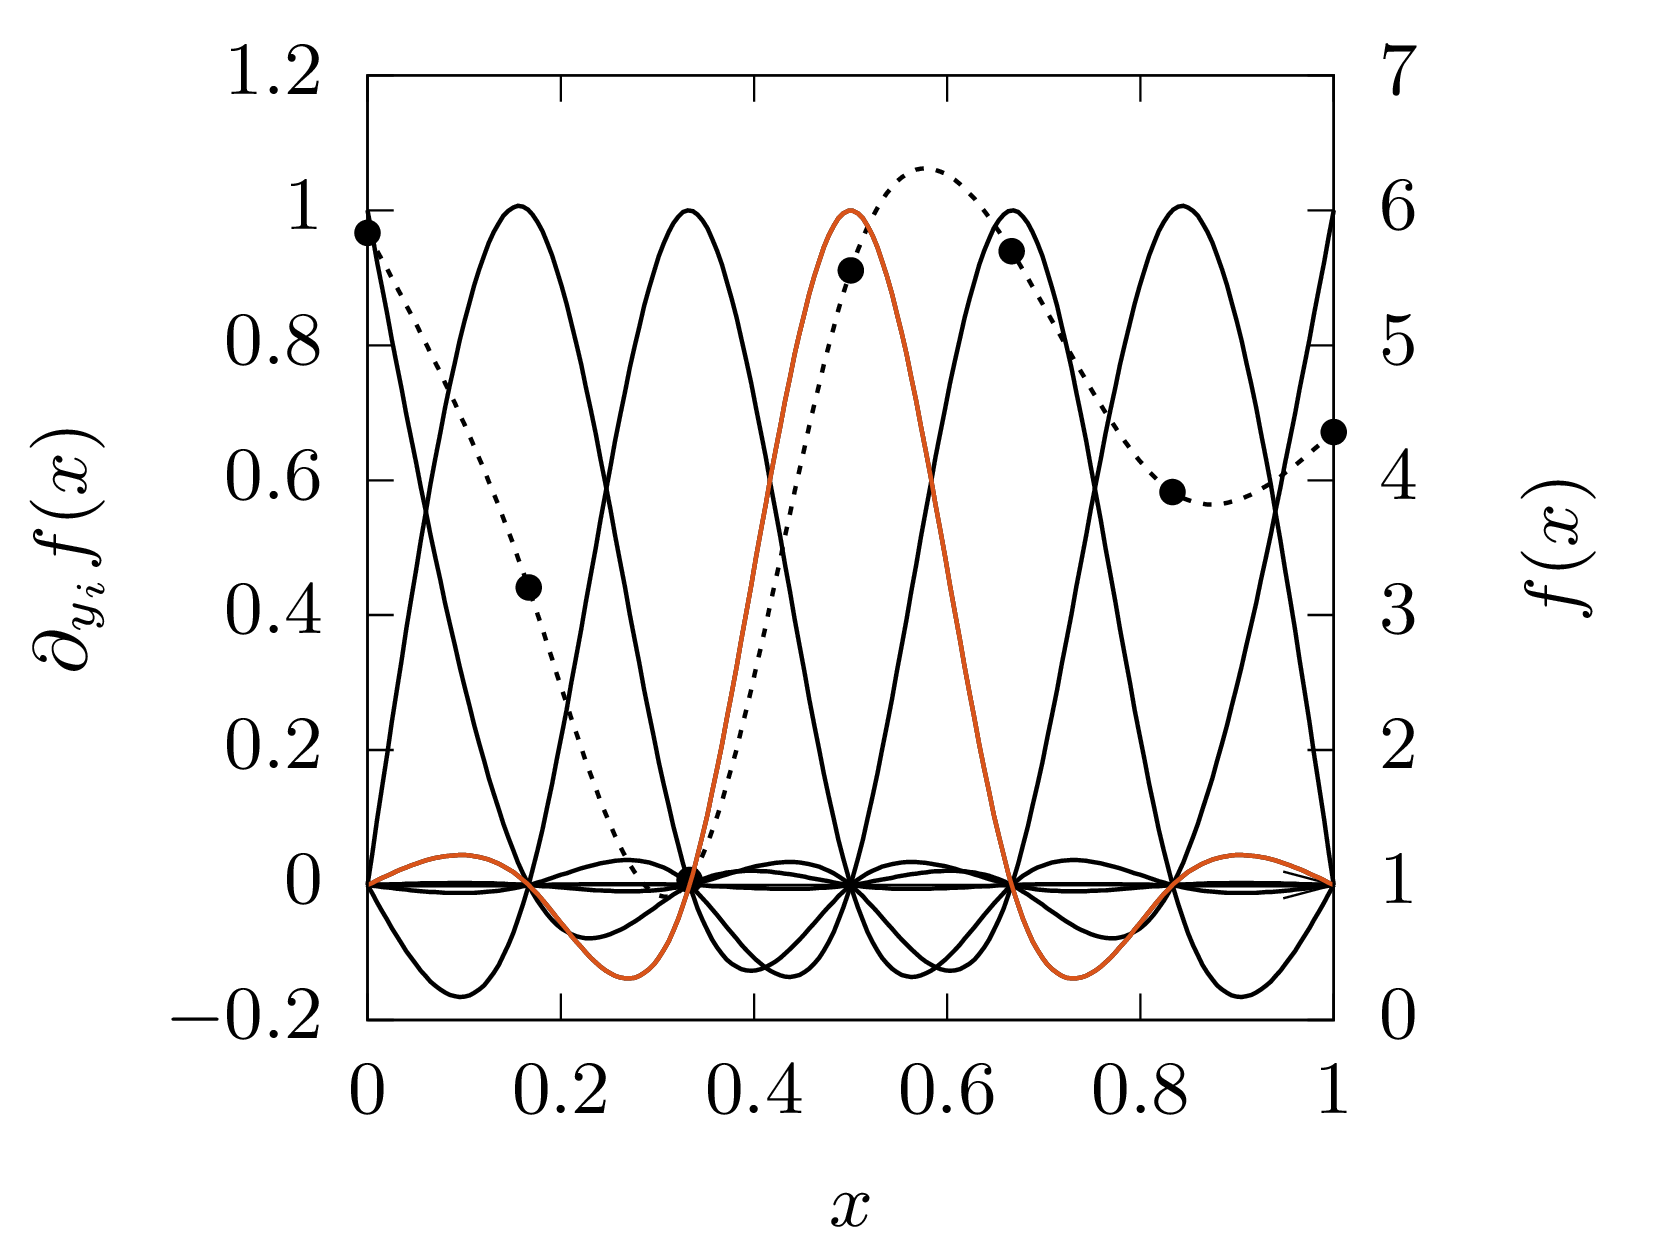
\includegraphics[scale=1.]{cspline/spline.png}
    \caption{Natural cubic spline (dashed line, right axis) of $n=7$ equidistant $(x_i, y_i)$ tuples (dots, right axis), as well as its derivatives w.r.t.\ $y_i$ (solid lines, left axis).}
    \label{fig:cspline_derivs}
\end{figure}

We note once more that $q_{ij}$ is not a function of $y_i$ and is unambiguously defined by $n$.
This is also given for other expansions of $f_i$ w.r.t.\ the grid points, for instance in the \textit{sinc-interpolation}
\begin{equation*}
    f_i(t) = \sum_{j=0}^k \operatorname{sinc}((t - j) \pi) y_j
\end{equation*}
which resembles the shape of the derivatives shown in Fig.~\ref{fig:cspline_derivs} in good approximation.
The expansion coefficients $q_{ij}$ of the sinc-interpolation do not even depend on $n$ anymore and there is no need to invert a $n \times n$ band matrix.
However, this computational benefit is compensated by the fact that sinc-interpolations tend to overshoot compared to the cubic spline approach, even if damped with a Gaussian function, as shown in Fig.~\ref{fig:cspline_sinc}.
\begin{figure}[htbp]
    \centering
    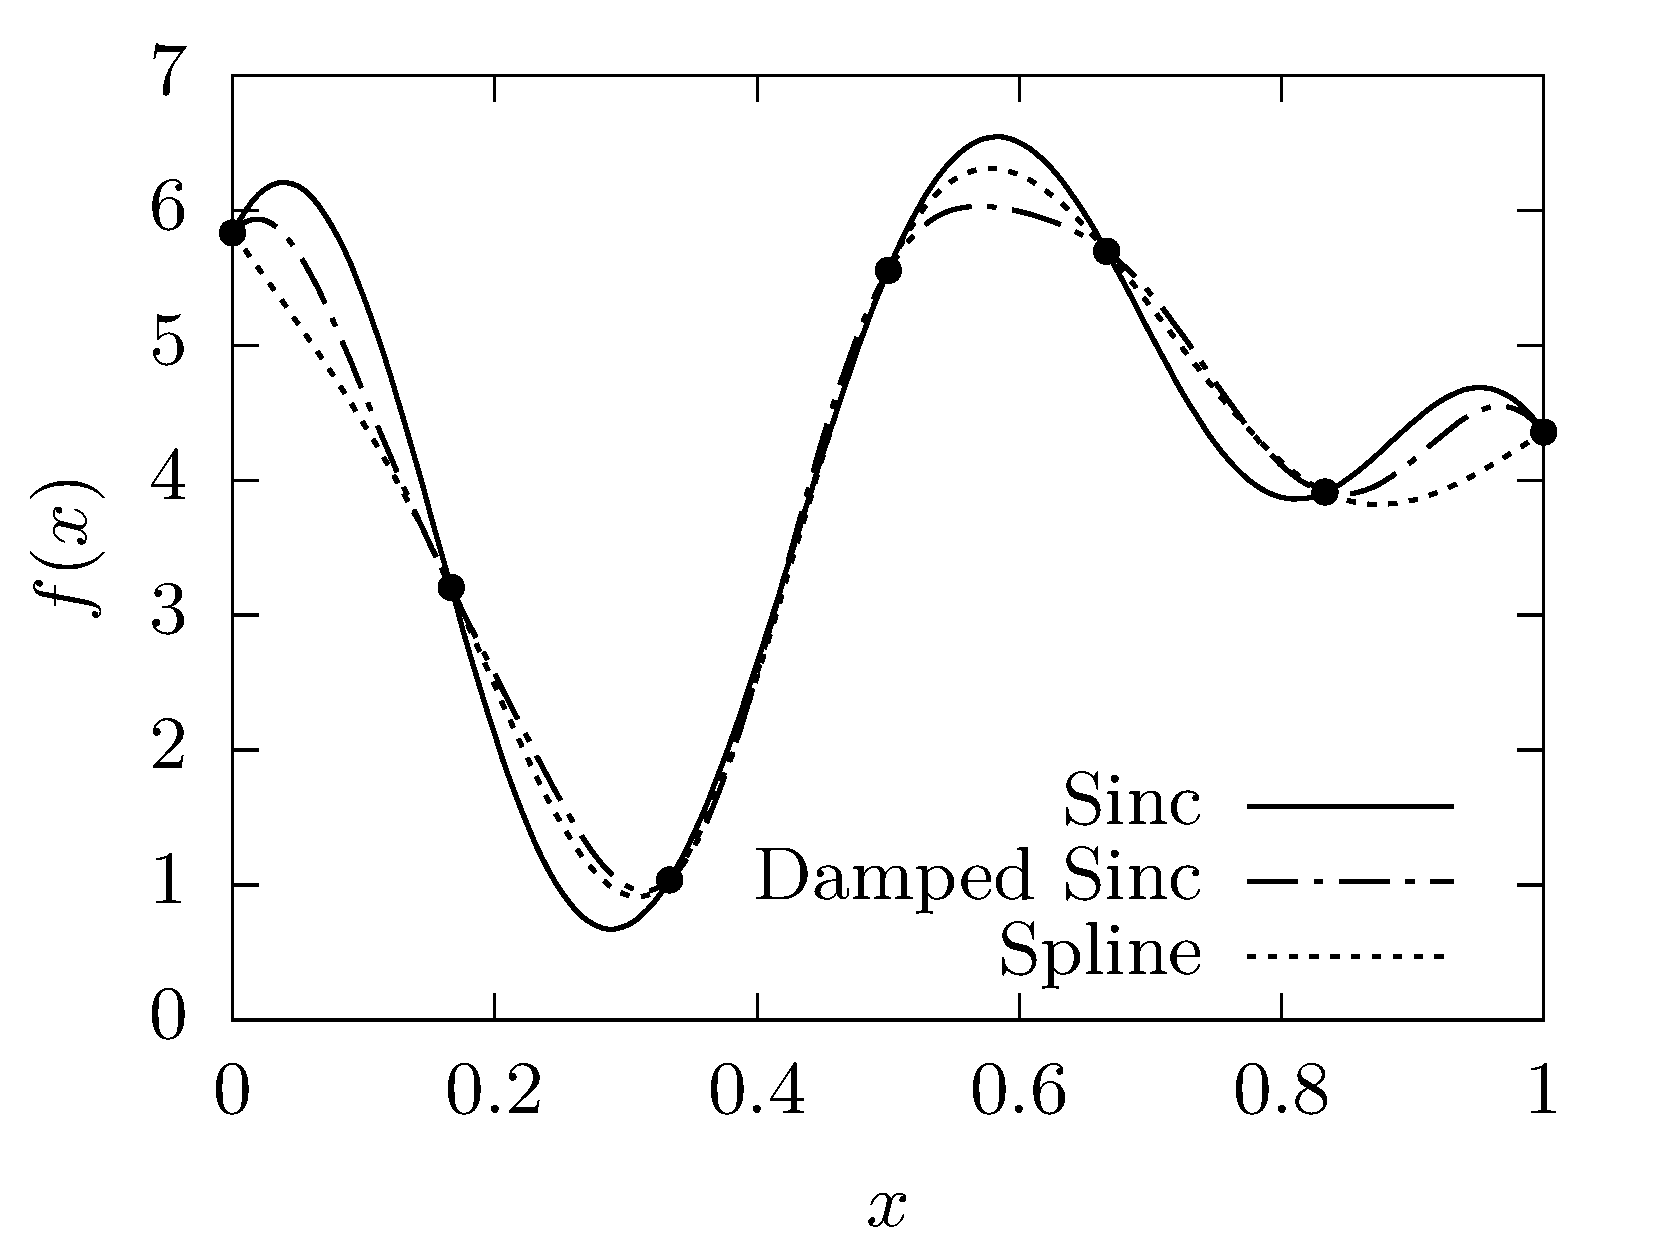
\includegraphics[scale=1.]{cspline/sinc.png}
    \caption{Sinc-interpolation w/o and with Gaussian damping ($\sigma=1$), as well as a natural cubic spline for $n=7$ equidistant $(x_i,y_i)$ tuples (dots).}
    \label{fig:cspline_sinc}
\end{figure}
